\documentclass{article}

% Language setting
% Replace `english' with e.g. `spanish' to change the document language
\usepackage[english]{babel}

% Set page size and margins
% Replace `letterpaper' with `a4paper' for UK/EU standard size
\usepackage[letterpaper,top=2cm,bottom=2cm,left=3cm,right=3cm,marginparwidth=1.75cm]{geometry}

% Useful packages
\usepackage{amsmath}
\usepackage{graphicx}
\graphicspath{ {./images/} }
\usepackage[colorlinks=true, allcolors=blue]{hyperref}

\title{Google TPU}
\author{Fernando Lima \\ Isabella Caselli \\ Rodrigo Michelassi}

\begin{document}
\maketitle

\begin{abstract}
Na era do desenvolvimento de sistemas baseados em Inteligência Artificial, se faz necessário o uso de máquinas super potentes, capazes de processar dados e realizar operações matemáticas de maneira extremamente rápida. Modelos de Machine Learning podem levar horas, até mesmo dias, para serem treinados, devido principalmente a operações como produto interno entre matrizes e a enorme quantidade de dados que são usados, trazendo um prejuízo não apenas de tempo, mas também energético, ambiental e sobretudo lucrativo. Nesse artigo, iremos tratar brevemente sobre a utilização de Cloud TPUs, unidades de processamento de tensores do Google Cloud, que atuam na otimização do treinamento de modelos de aprendizado de máquina, e que se tornou indispensável na academia e na indústria, para todos estudiosos e profissionais da área.
\end{abstract}

\section{Introdução}

\section{History}

\subsection{Tensores}

\subsection{Modelos de Aprendizado de Máquina}

\section{Arquitetura da TPU}

\section{TPU vs GPU}

\section{TensorFlow}

\section{Cloud TPU v5p}

Como discutido anteriormente, LLMs são os novos modelos mais explorados no mercado e na academia. Todavia, esses modelos utilizam dados de toda (ou quase toda) a internet, que cresce ainda mais exponencialmente. Todos os dias há milhões de novos dados sendo gerados. Dessa forma, é importante que o hardware acompanhe o crescimento na quantidade de dados disponíveis, de forma que seja possível possuir poder computacional suficiente para treinar modelos como esses.

Com isso em vista, a evolução das TPUs deve ser rápida, portanto, em 2023, a Google apresentou, em 2023, a v5p, a TPU mais poderosa da empresa. Com esse lançamento, a Google prometeu a entrega de uma performance até $2.8$ vezes mais rápida, utilizada para alimentar ecossistemas internos da multinacional, como o Youtube, Android e Gmail.

Essa TPU se diferencia das demais, pois é focada em desempenho possível, sem levar em consideração a facilidade operacional. Um grande diferencial é a forma como a TPU lida com operações em ponto flutuante. Por dados oficiais da Google, essa arquitetura traz $8960$ chips e três vezes mais memória HBM.

\begin{figure}[h]
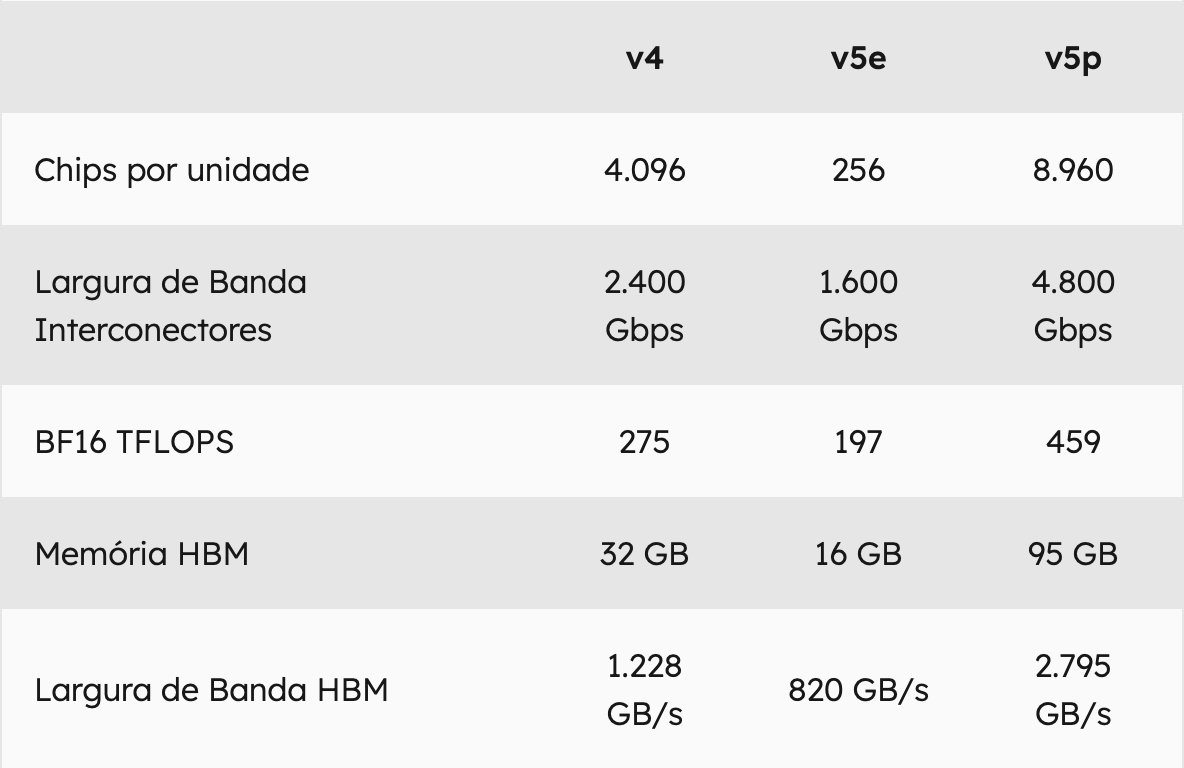
\includegraphics[scale=0.5]{comparativo-tpus}
\centering
\caption{Comparativo entre TPUs Google para cargas de trabalho em IA e LLM}
\end{figure}

Mas no fim, o que significam esses valores? A Google promete que a nova TPU consegue escalar o tempo de treinamento, sendo até $4X$ mais rápida que TPUs mais baratas, como a $V4$, devido ao dobramento no tamanho de operações em ponto flutuante que são entregues.

\section{Google Colab e distribuição}

\bibliographystyle{alpha}
\bibliography{sample}

\href{https://www.run.ai/guides/cloud-deep-learning/google-tpu}{TPU e Arquitetura}

\href{https://cloud.google.com/blog/products/compute/performance-per-dollar-of-gpus-and-tpus-for-ai-inference}{Comparativos oficiais em modelos de IA (TPU vs GPU)}

\href{https://canaltech.com.br/inteligencia-artificial/cloud-tpu-v5p-e-o-novo-e-mais-poderoso-acelerador-de-ia-do-google-272299/}{TPU v5p}

\href{https://cloud.google.com/tpu?hl=pt-BR}{Conceitos básicos}

\href{https://en.wikipedia.org/wiki/Tensor_Processing_Unit}{Wikipedia, tem tudo}

\end{document}